\documentclass[a4paper]{article}
\usepackage{graphicx,wrapfig}
\usepackage{enumerate}
%\usepackage{proof} %for inference rules
\usepackage{amsmath} %for align
\usepackage{amssymb} %for a proper-sized entailment sign (\rhd)
\usepackage{times} %for better looking font
\usepackage[usenames]{color} %for colored text
%\usepackage{arydshln} %for dashed lines in tables
\usepackage{float} %for boxes 
\usepackage[hang,small,bf]{caption}  %makes captions bold
\usepackage[a4paper=true, bookmarks=true, linkcolor=blue, citecolor=blue, urlcolor=blue, colorlinks=true, breaklinks=true, bookmarksopen=true]{hyperref} %must be at the end
\usepackage[all]{hypcap} %must be truly at the end, immediately after hyperref

\textwidth = 440pt 
\oddsidemargin = 0.2cm

%\setlength{\parindent}{0pt} 
\setlength{\parskip}{1ex plus 0.5ex minus 0.2ex} %set paragraph interspacing


\title{Knowledge Management for Twelf \\[5cm]
				\large{Master Thesis Proposal}}
\vspace*{3cm}
\author{\Large{Alin Iacob}}
\date{\today}

\newcommand{\eqwnos}[2] {			%a new equation WITHOUT numbers
	\begin{equation*}
		\label{#1}
		#2
	\end{equation*} }

\newcommand{\myref}[2] {			%proper hyperreference
  \hyperref[#2]{#1~\ref{#2}} }

\newcommand{\mmt} {\textsc{Mmt }}  % MMT in small caps
\newcommand{\openmath} {\textsc{OpenMath }}
\newcommand{\omdoc} {\textsc{OMDoc }}
\newcommand{\mathml} {\textsc{MathML }}

\newcommand{\calculus}[3] {		%list of unnumbered equations within a box, within a figure
				\begin{figure}[ht]    % !NO empty lines anywhere inside!
					\centering
					\begin{equation*}
 						 \addtolength{\fboxsep}{5pt}
   					 \boxed{
   							\begin{gathered}
   								#3
   							\end{gathered}  
   					 }
					\end{equation*}
  				\caption{#1}
  				\label{#2}
				\end{figure}
}

\newcommand{\nextinf}{\\ {} \\}		%next inference in a \calculus
\newcommand{\blue}[1] {	%easy coloring in blue
	\textcolor{blue}{#1}}

\newcommand{\set}[1] {\left\{ {#1} \right\}}
\newcommand{\pset}[2] {\left\{ {#1} ; {#2} \right\}}


\begin{document}
\maketitle
%\newpage
\newcommand{\ttt}[1]{{\tt #1}}

\section{Introduction}

The LATIN (Logic Atlas and Integrator) project~\cite{LATIN:url} focuses on developing a foundationally unconstrained framework for knowledge representation that allows to represent the meta-theoretic foundations of the mathematical knowledge in the same format and to interlink the foundations at the meta-logical level. 

Currently, the project consists in building an Atlas of Logics used in automated reasoning, mathematics, and software engineering concentrating on paradigmatic logics from first-order logic (TPTP, CASL, and Mizar), higher-order logics (PVS, Isabelle/HOL, HasCASL), and logical frameworks (LF and Isabelle). In order to provide a comprehensive logical framework, LATIN extends the Twelf language with a module system inspired by MMT~\cite{RabKoh:WSMSML10}.

As the Atlas of Logics grows in size and complexity, the need for adequate knowledge management becomes apparent. The next section presents a simplified version of the Twelf language with the MMT extensions, and sections~\ref{sec:shallow} and~\ref{sec:deep} describe two kinds of changes that allow for easier understanding of the Atlas and increase sustainability of a large code base.\cite{TISCAF}

In the last part of the report we present the details of the parser implementation (section~\ref{sec:code}) and the changes to the propositional logic tree (section~\ref{sec:pl})


\section{Preliminaries}\label{sec:preliminaries}

A file in the Atlas has the extension {\tt .elf} and is a collection of \textit{signatures} and \textit{views}.
\begin{enumerate}
\item A \textit{signature} is a list of \textit{symbol declarations} and \textit{structures}
\begin{verbatim}
%sig signature-name = {
  (symbol-declaration | structure-declaration)*
}
\end{verbatim}
where {\tt (A|B)*} indicates 0 or more occurrences of A or B.
	
	\begin{enumerate} 
	
	\item \textit{symbol declarations} are the core of the original Twelf language. They introduce new well-typed symbols.
\begin{verbatim}
symbol-name [: symbol-type] [= symbol-definition].
\end{verbatim}
where square brackets indicate that their contents is optional. At least one of \{symbol-type, symbol-definition\} must be given for each symbol. Each of \{symbol-type, symbol-definition\} is a well-formed expression with atoms declared earlier.
	
	\item \textit{structures} have the (simplified) form
\begin{verbatim}
%struct struct-name : domain = { 
   (symbol-name := expression.)*
}.
\end{verbatim}
A structure is equivalent to redeclaring all the symbols from the domain signature into the current signature, possibly with different definitions, as specified by the {\tt expressions}. 

The following restrictions are in place:
	\begin{itemize}
	\item {\tt domain} is an already declared signature name.
	\item the set of {\tt symbol-names} is a subset of the names without definiens declared in {\tt domain}. The symbols from the domain signature which are not assigned to anything in the {\tt structure} are simply imported as-is into the current signature.
	\item each {\tt expression} is formed using only symbols declared earlier in the parent signature.
	\end{itemize}
	A symbol available as {\tt symbol-name} in the {\tt domain} can be used within expressions in the current signature as {\tt struct-name.symbol-name}.
	
	\item An \textit{import} is syntactic sugar for a structure declaration with empty body, where every symbol from the domain is imported as-is into the current signature.
\begin{verbatim}
%include domain.
\end{verbatim}
A symbol available as {\tt symbol-name} in the {\tt domain} can be used within expressions in the current signature as {\tt domain.symbol-name}.

	\end{enumerate}

\item A \textit{view} between two signatures has the (simplified) form
\begin{verbatim}
%view view-name : domain -> codomain = { 
   (symbol-name := expression.)*
}.
\end{verbatim}
	The following restrictions are in place:
	\begin{itemize}
	\item {\tt domain} and {\tt codomain} are already declared signature names.
	\item the {\tt symbol-names} are precisely the names without definiens declared in {\tt domain}.
	\item each {\tt expression} is formed using only symbols from {\tt codomain}.
	\end{itemize}
       	 Unlike structures, a \textit{view} does not add symbols to a signature. Its role is independent from those of the structures. If we regard signatures as mathematical theories, where axioms are encoded as symbols according to the Curry-Howard isomorphism, then a \textit{view} encodes an {\tt is-a} relation between {\tt codomain} and {\tt domain}.

Once we have a view from {\tt domain} to {\tt codomain}, every expression over the {\tt domain} can be translated (via structural induction, using the view assignments for the atoms) into an expression over the {\tt codomain}. Mathematically, any constructions or theorems of the {\tt domain} theory can be automatically translated to constructions and theorems of the {\tt codomain}.

\end{enumerate}

As signatures import symbols via \ttt{\%struct} and \ttt{\%include} statements, it is fitting that views and structure bodies have a way to directly map these inclusions to some existing morphism (i.e. composition of views and/or structures), instead of having to map each induced symbol to an expression. Morphisms are thus defined as: \ttt{(struct-name | view-name)*}, where concatenation means composition. 

Accordingly, one can use the construct
\begin{verbatim}
%struct struct-name := morphism.
\end{verbatim}
inside both views and \ttt{\%struct} declarations, and
\begin{verbatim}
%include view-name.
\end{verbatim}
inside views.

For examples and more explanations, see Section 3 in~\cite{rabeEA:twelfmod:09}.


\section{Shallow improvements}\label{sec:shallow}
\subsection{Problems with existing knowledge management in the Logic Atlas}
The Logic Atlas is organized via a standard file system directory
tree. Each component (or module) resides in a file, while the
hierarchy of organization is encoded via the directory structure of
the project. Each resource in the atlas is assigned a global URI\footnote{such as \ttt{http://cds.omdoc.org/logics/first-order/syntax/base.elf}} by an external convention (it coincides with the URL on a university server on which an official copy resides). Once the Atlas is checked out via SVN, the physical location becomes file-system specific\footnote{such as 
\ttt{file:/c:/courses/twelf/logics/first-order/syntax/base.elf}} and does not coincide with the (globally-unique) URI any more.

The current structure of the Logical Atlas consists of a multi-tier
hierarchy, where:
\begin{enumerate}
\item On the top level we distinguish between the different scientific
  domains that define their own, interrelated system of logics and
  theories. At the moment of writing, these fields are
  \ttt{logics}, \ttt{math}, \ttt{category\_theory},
  \ttt{set\_theories}, \ttt{type\_theories}, and \ttt{translations}. A problem with the current organization at this level is
  the inclusion of non-atlas content into the repository,
  namely \ttt{admin}, \ttt{projects} and \ttt{unsorted}
  directories. Ideally, those should be kept in a separate
  repository as they violate the hierarchy principles and integrity of the LATIN library.
\item The next level (depth 2) models a classification of
  subdomains, for the specific field given at depth 1. For example,
  for \ttt{logics} there exist \ttt{first-order} and \ttt{higher-order}
  subclasses, while for \ttt{math} currently there are \ttt{algebra} and
  \ttt{relations}. 

  However, there is no limitation on the number of intermediate levels
  that can be modeled by this directory tree - while the 
  \ttt{math} field has a single level of subdomains, the
  \ttt{logics} field has two. Naturally,
  the depth of the intermediate directories will grow alongside the
  refinement of granularity of the library.
\item The leaf level contains the logics (or fragments thereof)
  as \ttt{.elf} files, as explained in Section~\ref{sec:preliminaries}. Each of those fragments is, however,
  not self-contained, but has dependencies in different files from the same logic, in other logics, and even in other depth 1 folders of the hierarchy - set theories and type theories.
\end{enumerate}


\subsection{Alleviatory measures}

\subsubsection{Metadata in comments}

In order to facilitate a management-friendly workflow of creating, maintaing and reorganizing modules, we propose the practice of adding commentary headers to every physical file, containing the following information:
\begin{itemize}
\item List of authors
\item File license
\item Description of the file purpose
\item Anything else the author deems important
\end{itemize}
Comments like this, containing useful metadata, will be enclosed by \ttt{\%* ... *\%} instead of the usual multi-line \ttt{\%\{ ... \}\%} or single-line \ttt{\%\%}. Each property like author or license will be written as a key-value pair:
\begin{verbatim}
@key_name  value_string
\end{verbatim}
where \ttt{key\_name} is user-definable, in order to accommodate for as much diversity as possible.

Furthermore, each module shall have a similar comment before. The first 0 or more lines of the comment contain key-value pairs. Starting from the next line, the first sentence is considered to be a ``short description'' of the module that follows and, together with the rest of the sentences (if they exist), it forms the ``long description''. Similar to Javadoc, this distinction allows code editors to show both small captions with information about a module and larger help boxes if needed.

\subsubsection{Over-modularity}

On level 3 and 4 of the logic graph, most logics have a folder each for syntax, proof theory, model theory and soundness. Furthermore, each folder contains many files, most of which have a small number of modules, but which are highly dependent on each other and on other files and folders. This has proved to be exceedingly confusing for beginners trying to understand the structure of the Atlas, or even trying to understand the dependencies of a single module, which can already be as many as 8 levels deep. 

An improvement for understanding is to group the syntax modules in one file, the proof theory in another, etc. Section~\ref{sec:pl} shows how this has been done for Propositional logic, greatly reducing the complexity of the dependency graph, while keeping the readability of the code.

\subsubsection{Under-modularity}

In some places within the logic graph, two logics are implemented in the same folder, each of them split into several files, making it difficult to see at a glance which files are part of which logic. An example of this is Minimal propositional logic and ``normal'' propositional logic. In this case, we have split the two logics into different folders. Nevertheless, this is not always the best approach, as seen with Intuitionistic propositional logic and Classical propositional logic, the latter of which is a small extension of the first. Both of them belong in the same place, since one is only defined in terms of another.

Same problems are often encountered with two model theories mixed in one folder. Since they belong to the same logic, they should stay there, but in separate subfolders, as they do not depend on each other.



\section{Deep improvements}\label{sec:deep}

\subsection{Read statements versus namespaces}

\subsubsection{Problem}

\ttt{\%read} declarations make all the imported module names visible in the entire file scope, which leads to possible name clashes, since modules written in different parts of the graph may have the same name. The existing approach for avoiding this is to append prefixes and/or suffixes to each module name, in order to make them as globally unique as possible, so as to avoid any possible clash when someone uses them in conjunction with another file. The result is names that are too long and artificial, with modules like \ttt{Forall}, \ttt{ForallPF}, \ttt{ForallPFExt} or \ttt{Bool} vs \ttt{Boolean}. In the future, as the Atlas expands, it becomes unfeasible for  authors to invent unique names for their modules, since they would have to look through the entire repository. Even if they have tools to automate this, the resulting long names will make the code unreadable.

\subsubsection{Solution}

Namespaces offer a solution: each file shall have a ``current'' namespace declaration immediately after the initial comment:
\begin{verbatim}
%namespace "absolute namespace uri"
\end{verbatim}
This namespace is required to be globally unique URI and for the time being, this is accomplished by having it reside in the subdirectory tree of \ttt{http://cds.omdoc.org/}, where it will presumably be uploaded via SVN. Documents can only reference each other by knowing this URI.

The \ttt{\%read} statements are replaced by 
\begin{verbatim}
%namespace alias = "foreign uri"
\end{verbatim}
where \ttt{alias} is an identifier and \ttt{uri} is a relative uri based on the last ``current'' namespace declaration. From the point of the alias declaration onwards, a module \ttt{A} declared within the scope of the ``foreign uri'' \ttt{U} can be referred to as \ttt{U.A}.

Namespaces are already defined conceptually, but there is no tool to support them yet.


\subsection{A catalogue service}

\subsubsection{Problem}

In the current setup, the namespace alias declarations present a conceptual dead-end for automated knowledge
  management, because the author-defined namespace hierarchy does not necessarily correspond to the physical, system-understandable file URLs. The  synchronization of the two types of orderings can be achieved only  by tedious efforts, which is a strong motivation for automatizing it.

To make the problem worse, each file can contain references to any number of other namespaces, allowing for
various kinds of inconsistencies, such as circular imports and hierarchy violations. Detection can be done with graph algorithms.

A catalogue infrastructure that translates from URI (namespaces) to URL (filenames) has been designed, but not implemeneted. 

\begin{itemize}
\item URIs are logical references. The Twelf files contain only logical references, not physical references
\item URLs are physical references. Such a catalogue cannot be in the SVN repository, hence every user who checks out from the server needs to set their own catalogue.
\end{itemize}

We provide tool support to perform this translation and to create the catalogue.

\subsubsection{Solution}

We implemented a parser called \ttt{crawler} which harvests the information given by \ttt{\%namespace}, \ttt{\%include}, \ttt{\%struct}, domains and codomains of views and generates an XML file that offers, for each module, its URI, URL and a list of dependencies given as URIs. All the URI and URLs are absolute. Thus, the generated file can function as a catalogue translating URIs to URLs.

The parser also gathers metadata information from the comments described in~\ref{sec:shallow}, for the files as well as for the modules.

While the parser is described extensively in section~\ref{sec:code}, below are a few example of Twelf input with the corresponding XML output.

\begin{enumerate}[\textit{Example 1.}]
\item The Twelf+MMT code present from file \ttt{L/classic/proof\_theory.elf}
\begin{verbatim}
%*
   @author Fulya Horozal, Florian Rabe
   @license LATIN
   Signature for proof theory of Classical propositional logic
*%

%namespace "I/classic/proof_theory.elf".
%namespace syntax = "syntax.elf".

%* true introduction *%
%sig Truth = {
  %include syntax.Truth    %open.
  trueI  : ded true.
}.

%* false elimination *%
%sig Falsity = {
  %include syntax.Falsity  %open.
  falseE : ded false -> {A} ded A.
}.
...
\end{verbatim}
is mapped to
\begin{verbatim}
<?xml version="1.0" encoding="UTF-8"?>
<skeleton>

   <document URL="L/classic/proof_theory.elf">
      <meta>
         <author>Fulya Horozal, Florian Rabe</author>
         <license>LATIN</license>
         <short>   Signature for proof theory of Classical 
                      propositional logic</short>
      </meta>
      <dependency URI="I/classic/syntax.elf" />
   </document>

   <sig URI="I/classic/proof_theory.elf?Truth" 
          URL="L/classic/proof_theory.elf#position(10;0;13;1)">
      <meta>
         <short> true introduction </short>
      </meta>
      <dependency URI="I/classic/syntax.elf?Truth">
   </sig>

   <sig URI="I/classic/proof_theory.elf?Falsity"  
          URL="L/classic/proof_theory.elf#position(16;0;19;1)">
      <meta>
         <short> false elimination </short>
      </meta>
      <dependency URI="I/classic/syntax.elf?Falsity">
   </sig>
   ...
</skeleton>
\end{verbatim}
In order for the examples to fit in the page, we used the shortcuts 
\begin{itemize} 
\item \ttt{I}  instead of  \ttt{http://cds.omdoc.org/logics/propositional} and
\item \ttt{L} instead of \ttt{file:/C:/courses/Twelf/logics/propositional}.
\end{itemize}


\item[\textit{Example 2.}]  The Twelf+MMT code from file \ttt{file:/C:/courses/Twelf/logics/meta/bool-zf.elf}
\begin{verbatim}
%*
   @author Florian Rabe
   @license LATIN
   View from (Booleans in STTIFOL) to (Booleans in ZF)
*%

%namespace "http://cds.omdoc.org/logics/meta/bool-zf.elf".
%namespace bool_sttifol = "bool.elf".
%namespace bool_zf = "../../set_theories/zfc/bool.elf".
%namespace sttifol-zf = "sttifol-zf.elf".

%view Bool-ZF : bool_sttifol.Bool -> bool_zf.Boolean = {
   %include sttifol-zf.STTIFOLEQ-ZF.
   bool' := cbool.
   0     := ⊥.
   1     := ⊤.
   cons  := ccons.
   boole := ctnd.
   ...
}.
\end{verbatim}
is mapped to
\begin{verbatim}
<?xml version="1.0" encoding="UTF-8"?>
<skeleton baseURI="http://cds.omdoc.org/logics/meta/" baseURL="">

   <document URL="file:/C:/courses/Twelf/logics/meta/bool-zf.elf">
      <meta>
         <author>Florian Rabe</author>
         <license>LATIN</license>
         <short>   View from (Booleans in STTIFOL) to (Booleans in ZF)</short>
      </meta>
      <dependency URI="http://cds.omdoc.org
                                             /logics/meta/bool.elf" />
      <dependency URI="http://cds.omdoc.org
                                            /set_theories/zfc/bool.elf" />
      <dependency URI="http://cds.omdoc.org
                                            /logics/meta/sttifol-zf.elf" />
   </document>

   <view URI="http://cds.omdoc.org/logics/meta/bool-zf.elf?Bool-ZF"
             URL="file:/C:/courses/Twelf/logics
                              /meta/bool-zf.elf#position(11;0;21;1)">
      <dependency URI="http://cds.omdoc.org/logics
                                       /meta/bool.elf?Bool">
      <dependency URI="http://cds.omdoc.org/set_theories
                                       /zfc/bool.elf?Boolean">
      <dependency URI="http://cds.omdoc.org
                            /logics/meta/sttifol-zf.elf?STTIFOLEQ-ZF">
   </view>

</skeleton>
\end{verbatim}
\end{enumerate}



\section{Interface}\label{sec:interface}

\subsection{Web server}

The \ttt{crawler.Run} object starts a RESTful\footnote{\url{http://en.wikipedia.org/wiki/Representational\_State\_Transfer\#RESTful\_web\_services}} web server on localhost. 

\subsubsection*{Command-line arguments}

\ttt{crawler.Run} accepts the following command-line arguments:

\begin{center} \ttt{crawler.Run (--port port\_number)? (location|+pattern|-pattern)*} \end{center}

\begin{itemize}
\item \ttt{--port} \  \textit{port number} \\ 
        The port number on which the server runs. This argument is optional and must be the first. The default port number is 8080 (historically a common choice for web servers operated in non-root mode\footnote{GRC - Port Authority, \url{http://www.grc.com/port\_8080.htm}}).
\item \textit{location} \\
	Absolute path to a file or directory in the local file system. The program continuously and recursively crawls these locations and updates the hashes with the information from them. 

\item \ttt{+}\textit{pattern} \\
        An inclusion pattern, where \textit{pattern} is a file or directory name, without its path. The star (*) is the only special character and matches any sequence of characters.

\item \ttt{-}\textit{pattern} \\
        An exclusion pattern.

       Inclusion and exclusion patterns affect which files and folders are crawled recursively, starting from the locations provided as command-line arguments and, later, given by web requests:
	\begin{enumerate}
	\item  Folders are crawled if they do not match any exclusion pattern.
	\item  Files are crawled if they match at least one inclusion pattern, but no exclusion pattern. \\ If no inclusion patterns are provided, only the second condition remains. 
	\end{enumerate}
\end{itemize}


\subsubsection*{Administration web page}

The web server provides a page (Figure~\ref{fig:admin}) where the user can add inclusion/exclusion patterns and locations, and see the existing ones. There is also the possibility to re-crawl all the locations and to shutdown the server. 

\begin{figure}
  \begin{center}
     \fbox{
       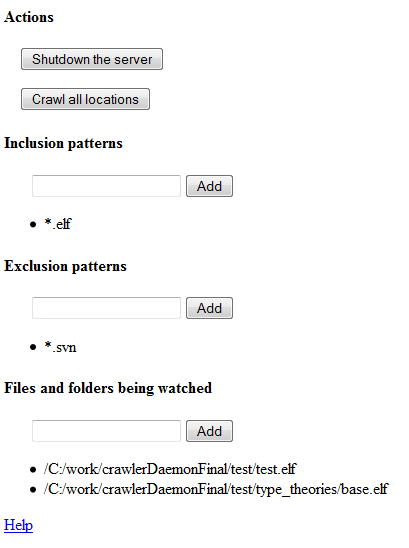
\includegraphics[width=7cm]{admin.png}
     }
  \end{center}
  \caption{Web administration interface (\url{http://localhost:8080/admin})}
  \label{fig:admin}
\end{figure}


\subsubsection*{GET requests and responses}

\begin{enumerate}
\item \textbf{Get metadata as text} \qquad  \ttt{/getMetaText?uri=}\textit{entityUri}
	\begin{itemize}
	\item Print verbatim the semantic comment associated with an entity. \textit{entityUri} can be either a file path, in which case the document metadata is returned, or the URI of a module, constant or structure declaration. If the entity does not have a semantic comment associated with it, an empty text is returned. If \textit{entityUri} is neither a valid URI, nor a file path already in the list of locations, then an error message is returned.
	\item \textit{Example:} 
		\begin{itemize}
		\item Request URL:  \url{http://localhost:8080/getMetaText?uri=C:/modules-lambda.elf}
		\item Response: 
		\begin{verbatim}Some orthogonal features of type theories occurring in the lambda cube
   @author Fulya Horozal, Florian Rabe\end{verbatim}
		\end{itemize}
	\item \textit{Example:} 
		\begin{itemize}
		\item Request URL:  \url{http://localhost:8080/getMetaText?uri=http://cds.omdoc.org/type\_theories/modules-lambda.elf?DepFun?@}
		\item Response: 
		\begin{verbatim}elimination\end{verbatim}
		\end{itemize}
	\end{itemize}


\item \textbf{Get metadata as OMDoc} \qquad  \ttt{/getMeta?uri=}\textit{entityUri}
	\begin{itemize}
	\item Print the semantic comment associated with an entity, as OMDoc. The comment is parsed as follows: The first line of the comment is the ``short'' comment, which can be used for example as a hover text in an IDE. Starting from the second line is the ``long'' comment, which is intended to be an elaboration of the short comment. 

The first line that starts with ``@'' is a key-value property line. ``@'' must be followed by a word of non-zero length, which will be the key. The key and value are separated by whitespace, and the value starts at the first non-whitespace character and ends before the line separator. After a key-value property line, all the lines must be key-value properties. The key-value properties may start on the first or second line, i.e. the ``short'' and ``long'' comments are optional.

 \textit{entityUri} can be either a file path, in which case the document metadata is returned, or the URI of a module, constant or structure declaration. If the entity does not have a semantic comment associated with it, an empty text is returned. If \textit{entityUri} is neither a valid URI, nor a file path already in the list of locations, then an error message is returned.
	\item \textit{Example:} 
		\begin{itemize}
		\item Request URL:  \url{http://localhost:8080/getMeta?uri=C:/modules-lambda.elf}
		\item Response: 
		\begin{verbatim}<metadata>
  <metadatum key="short">
    Some orthogonal features of type theories occurring in the lambda cube
  </metadatum>
  <metadatum key="author">Fulya Horozal, Florian Rabe</metadatum>
</metadata>\end{verbatim}
		\end{itemize}
	\item \textit{Example:} 
		\begin{itemize}
		\item Request URL:  \url{http://localhost:8080/getMeta?uri=http://cds.omdoc.org/type\_theories/modules-lambda.elf?DepFun?@}
		\item Response: 
		\begin{verbatim}<metadata>
  <metadatum key="short">elimination</metadatum>
</metadata>\end{verbatim}
		\end{itemize}
	\end{itemize}


\item \textbf{Get text} \qquad  \ttt{/getText?uri=}\textit{entityUri}
	\begin{itemize}
	\item Print verbatim the text of an entity. \textit{entityUri} can be either a file path, in which case the entire document is printed, or the URI of a module, constant or structure declaration. If \textit{entityUri} is neither a valid URI, nor a file path already in the list of locations, then an error message is returned.
	\item \textit{Example:} 
		\begin{itemize}
		\item Request URL:  \url{http://localhost:8080/getText?uri=http://cds.omdoc.org/type\_theories/modules-lambda.elf?DepFun?@}
		\item Response: 
		\begin{verbatim}@    : scope.exp (Π [x : domain.exp A] B x) -> {a : domain.exp A} scope.exp B a.\end{verbatim}
		\end{itemize}
	\end{itemize}


\item \textbf{Get OMDoc} \qquad  \ttt{/getOmdoc?url=}\textit{path}
	\begin{itemize}
	\item Print the Omdoc skeleton of a document given by its disk address. \textit{path} must be a file path. If \textit{path} is  not a file path already in the list of locations, then an error message is returned.
	\item \textit{Example:} 
		\begin{itemize}
		\item Request URL:  \url{http://localhost:8080/getOmdoc?url=C:/modules-lambda.elf}
		\item Response: 
		\begin{verbatim}<?xml version="1.0" encoding="UTF-8"?><omdoc 
base="http://cds.omdoc.org/type_theories/modules-lambda.elf" xmlns:om="http://www.openmath.org/OpenMath" xmlns="http://omdoc.org/ns">
  <metadata>
    <metadatum key="short">
      Some orthogonal features of type theories occurring in the lambda cube
    </metadatum>
    <metadatum key="author">Fulya Horozal, Florian Rabe</metadatum>
  </metadata>
  <theory 
  uri="http://cds.omdoc.org/type_theories/modules-lambda.elf?DepFun" name="DepFun">
    <metadata>
      <metadatum key="short">generalized dependent abstraction</metadatum>
    </metadata>
    <structure
    ...\end{verbatim}
		\end{itemize}
	\end{itemize}



\item \textbf{Get namespaces} \qquad  \ttt{/getNSIntroduced?url=}\textit{path}
	\begin{itemize}
	\item Print the namespaces introduced by the document given by its disk address. \textit{path} must be a file path. If \textit{path} is  not a file path already in the list of locations, then an error message is returned.
	\item \textit{Example:} 
		\begin{itemize}
		\item Request URL:  \url{http://localhost:8080/getNSIntroduced?url=C:/modules-lambda.elf}
		\item Response: 
		\begin{verbatim}http://cds.omdoc.org/type_theories/modules-lambda.elf\end{verbatim}
		\end{itemize}
	\end{itemize}


\item \textbf{Get dependencies} \qquad  \ttt{/getDependencies?uri=}\textit{entityUri}
	\begin{itemize}
	\item Print the URIs of the dependencies of an entity, one per line. \textit{entityUri} must be the URI of a module, constant or structure declaration. If \textit{entityUri} is not a valid URI, then an error message is returned.

The dependencies of a module are the imported modules, the domains of the structs declared and, for views, the domain and codomain. The only dependency of a structure declaration is its domain, and constant declarations have no dependencies.
	\item \textit{Example:} 
		\begin{itemize}
		\item Request URL:  \url{http://localhost:8080/getDependencies?uri=http://cds.omdoc.org/type\_theories/modules-lambda.elf?DepTypes}
		\item Response: 
		\begin{verbatim}http://cds.omdoc.org/type_theories/base.elf?KindsTypesTerms
http://cds.omdoc.org/type_theories/modules-lambda.elf?DepFun\end{verbatim}
		\end{itemize}
	\end{itemize}



\item \textbf{Get position} \qquad  \ttt{/getPosition?uri=}\textit{entityUri}
	\begin{itemize}
	\item Print the file path and position within the file of an entity. All the position information is encoded in an URL consisting of the file path, followed by a fragment part of the form
\begin{center} \ttt{\#((}\textit{firstLine}\ttt{,}\textit{firstCol}\ttt{),(}\textit{secondLine}\ttt{,}\textit{secondCol}\ttt{))}. \end{center} \textit{entityUri} must be the URI of a module, constant or structure declaration. If \textit{entityUri} is not a valid URI, then an error message is returned.
	\item \textit{Example:} 
		\begin{itemize}
		\item Request URL:  \url{http://localhost:8080/getPosition?uri=http://cds.omdoc.org/type\_theories/modules-lambda.elf?DepTypes}
		\item Response: 
		\begin{verbatim}/C:/modules-lambda.elf#((40,0),(46,1))\end{verbatim}
		\end{itemize}
	\end{itemize}

\item \textbf{Print capabilities} \qquad  \ttt{/}, \ \ttt{/help} \\
	Print the list of requests accepted by the server and their meaning.
\end{enumerate}

In addition to these requests conforming to the REST philosophy, the server accepts a number of requests which modify the state of the server. All of them redirect to the admin page and any possible errors are logged to standard output.

\begin{enumerate}
\item Re-crawl all locations  \qquad  \ttt{/crawlAll} \\
	Crawl again all locations recursively. Only the files that have changed since the last crawl are taken into consideration. This request is normally not needed, since the server crawls all locations periodically.

\item Add a location  \qquad  \ttt{/admin?addLocation=}\textit{path} \\
	Add a disk location to the list of watched locations. This operation is equivalent to adding a location via program arguments when starting the server.

\item Add an inclusion pattern  \qquad  \ttt{/admin?addInclusion=}\textit{pattern} \\
	This operation is equivalent to adding an inclusion pattern via program arguments when starting the server.

\item Add an exclusion pattern  \qquad  \ttt{/admin?addExclusion=}\textit{pattern} \\
	This operation is equivalent to adding an exclusion pattern via program arguments when starting the server.
\end{enumerate}




\subsection{Logging and error reporting}

The following events are reported to stdout:
\begin{itemize}
\item user adds a location
\item a newly added location is an ancestor or descendant of an existing location
\item user adds an inclusion/exclusion pattern
\item a file or folder in a watched location is modified, crawled for the first time or deleted
\item a syntax error is reached when crawling a file. Currently, any syntax error in a file causes the crawling of that file to be aborted and all the information already extracted to be dropped. In order to be useful for IDE operations like auto-completion or metadata in hover text, the crawler must instead be resilient to errors and at least keep the information extracted until the error. This is planned for the immediate future, as the modular structure of the parser makes it well-suited for this change.
\end{itemize}


\subsection{Scala/Java API}

\subsubsection{Storage}

Object \ttt{Storage} is the entry point of the API. It stores the information extracted from the files and has control methods for adding locations and patterns, crawling the stored locations, and getting the information.
\begin{enumerate}
\item \ttt{addStringLocation(locationName: String)}
\end{enumerate}
	

The scaladoc generated at \ttt{doc/index.html} in the project folder has a more detailed documentation of the API.



\section{Code}\label{sec:code}

The basic role of the parser is to take as input a Twelf file or a directory with Twelf files, scan them recursively and generate an XML ``skeleton'' document with metadata and dependency information about each file and each module inside it.  While reading each file, the parser checks for syntactical (but not type-theoretical) validity. Two important metadata generated is the URI and exact position within the file (URL) of each module. The rest of the metadata is taken from comments associated with the file or with individual modules and is generated by key-value pairs like \ttt{@license LATIN}, where the keys are user-definable. The file and module dependencies are given as absolute URIs. The dependencies are taken from structures and imports and, in the case of the views, also from the domain and codomain. 


The crawler is divided into a \ttt{FileCrawler} class and a \ttt{crawler} object, which can be run to crawl a directory or a file, by creating a new \ttt{FileCrawler}  for each file.  


\subsection{FileCrawler class}

\subsubsection{Data structures}

We will describe the datastructures  for organizing Twelf blocks defined in \ttt{FileCrawler} below:

\begin{enumerate}
\item {\tt BoundingBox}: stores initial and final coordinates of a block of text 
\item {\tt Block}: a generic block that will be extended with different case classes for modules, declarations, read statements, etc.
\item {\tt StringBlock}: stores coordinates of a string surrounded by double quotes, used for URIs given in the files
\item {\tt NamespaceBlock}: stores data about namespace declaratons, such as the namesace, URI and its alias
\item {\tt CommentProperty}: stores a key value property starting with an "@" symbol in a comment
\item {\tt CommentThrowBlock}: stores position of a comment with the syntax "\%\{ ... \}\%"
\item {\tt CommentKeepBlock}: stores a list of dynamically generated properties of a semantic comment, i.e a comment with special syntax, which means it provides metadata for the block, symbol or document, following it.
\item{\tt SigBlock}: stores information about a signature: its metadata, a list of its dependencies, its URI and URL
\item{\tt ViewBlock}: stores  information about a view: its metadata, a list of its dependencies, its URI and URL
\end{enumerate}

For each such data structure, we overwrite the method \ttt{ToString}, which converts all the information inside to an appropriate XML node.

The \ttt{FileCrawler} class stores, for each object of this class, the following public data structures for organizing a file:
\begin{itemize}
\item \ttt{file: File} the Twelf file handle for reading

\item \ttt{out: BufferedWriter} the file handle for buffered writing into \ttt{dependencies.xml}

\item \ttt{baseURI: URI} the URI against which the first namespace of the file is relative.

\item \ttt{baseURL: URI} the URL (folder location on local disk) which is the root of the file tree at \ttt{baseURI}.

\item \ttt{associatedComment: Block} the \ttt{\%* ... *\%} comment at the beginning of the file. If it doesn't exist, \ttt{associatedComment} remains \ttt{null}.

\item \ttt{fileURL: URI} file address on disk relative to \ttt{baseURL}.

\item \ttt{currentNS: URI} current namespace as absolute URI, against which each module URI is relative to. It is updated every time a \ttt{\%namespace "uri"} declaration is encountered.

\item \ttt{modules: ArraySeq[Block]} an array of \ttt{SigBlocks} and \ttt{ViewBlocks} extracted from the file

\item \ttt{deps: ArraySeq[URI]} an array of URIs for each dependency of the file, i.e. the set of namespace URIs declared in alias declarations. \ttt{deps} is equal to the set of values of the hash map \ttt{prefixes} (see below).

\end{itemize}

In addition to these, the class maintains several private data structures, useful for avoiding excessive message passing between various methods:

\begin{itemize}

\item \ttt{prefixes: HashMap[String, URI]} maps aliases to namespace URIs, as read from the \ttt{\%namespace alias = "uri"} declarations.

\item \ttt{lines: Array[String]} an array with the lines of the file in raw form

\item \ttt{flat: String} the flattening of \ttt{lines} into one String. Newlines are converted into spaces.

\item \ttt{lineStarts: ArraySeq[(Int, Int)]} keeps track of where each line starts. $(i, j) \in $\ttt{lineStarts} means that \ttt{flat}($i$) is the first character in the  $j$th line.

\item \ttt{keepComment: CommentKeepBlock} stores the most recent \ttt{\%* ... *\%} comment parsed. When the comment has been associated with a block, \ttt{keepComment} is set to \ttt{null}, in order to avoid associating comments to non-adjacent blocks.

\end{itemize}

Every file must start with a namespace declaration, either absolute or relative to \ttt{baseURI}. The software checks which case it is and, depending on whether a \ttt{baseURI} was given as program parameter, it computes the absolute URI or issues an error.

\subsubsection{Methods}

In addition to the datastructures, \ttt{FileCrawler} contains ``crawling'' methods which roughly correspond to each block type. Each such method reads a fragment of text starting from a position and returns a \ttt{Block} object with information extracted from the text. The methods check for syntactical well-formedness of the block and, in case of failure, throw a \ttt{ParseError} with a string explaining the reason of the error and the location inside the file where the error occurred. However, the methods assume that the correct block actually starts at the given position in the file; hence this must be ensured by the caller. 
\begin{enumerate}
\item \ttt{crawlString(Int): StringBlock} reads a double quoted string with the initial quotes at the given \ttt{Int} position. The \ttt{StringBlock} which is returned stores the string itself in the \ttt{name} field.

\item \ttt{crawlIdentifier(Int): Int} expects the first character of an identifier at the given position. An valid Twelf+MMT identifier:
	\begin{itemize}
	\item is at least one Unicode character long and can contain any Unicode characters, subject to the  restrictions below
	\item may contain dots, but not in its final position
	\item doesn't contain any character from the following: \ttt{()[]\{\}":\%}
	\item ends before a whitespace character or one of the forbidden character from the list above. It can end before a dot, only if that dot is followed by either a whitespace or one of the forbidden characters.
	\item is not identical to a reserved Twelf identifier: \ttt{->  <-  \_  =  type}
	\end{itemize}
	If the character at the starting position is already a forbidden character or a dot, a \ttt{ParseError} is thrown. If the identifier is a reseved Twelf identifier, a warning is printed, but the parsing continues.

	Unlike the other crawler methods, \ttt{crawlIdentifier} doesn't returns a special \ttt{Block} with the identifier, but simply returns the position immediately after the end of the identifier. The caller can then obtain the identifier by taking the substring between its initial and final position.

\item \ttt{crawlNamespaceBlock(Int): NamespaceBlock} reads both types of namespace declarations. For a declaration of type 
\begin{verbatim}
%namespace "uri"
\end{verbatim}
where \ttt{uri} is either an absolute uri (i.e. it is the first such declaration in the file), the method stores the name into \ttt{currentNS}. If \ttt{uri} is a relative uri based on the current namespace uri, the method updates \ttt{currentNS} by transforming the relative uri into an absolute one.

In the case of an alias declaration
\begin{verbatim}
%namespace alias = "uri"
\end{verbatim}
where \ttt{alias} is an identifier and \ttt{uri} is a relative uri based on the current namespace uri, the method converts the uri into an absolute one and updates the \ttt{prefixes} dictionary with the \ttt{(alias, absolute\_uri)} pair.

\item \ttt{crawlCommentThrowBlock(Int): CommentThrowBlock} reads a \ttt{\%\{ ... \}\%} comment and stores its start and end position.

\item \ttt{crawlCommentKeepBlock(Int): CommentKeepBlock} reads a \ttt{\%* ... *\%} comment and, for each line at the beginning starting with \ttt{@}, it parses the key and the value into a \ttt{CommentProperty} object, which is added to \ttt{CommentKeepBlock}'s \ttt{children} array.

\item \ttt{crawlSigBody(Int, SigBlock): Int} takes the position of the initial opening bracket of a signature body and the partially formed \ttt{SigBlock} object and parses each symbol declaration, \ttt{structure} and \ttt{import}. For the latter two, it computes the absolute uris of the domain signature and adds them to the \ttt{deps} (dependencies array) field of the parent \ttt{SigBlock} object.  \ttt{crawlSigBody} returns the position immediately after the final closing bracket.

\item \ttt{crawlSigBlock(Int): SigBlock} starts reading at the \ttt{\%} character from \ttt{\%sig}, checks for syntactical correctness and builds a \ttt{SigBlock} object by calling the \ttt{crawlSigBody} method.

\item \ttt{crawlViewBody(Int, ViewBlock): Int} takes the position of the initial opening bracket of a view body and the partially formed \ttt{ViewBlock} object and parses each assignment to symbol, assignment to structure and each import into the view. For the latter two, it computes the absolute uris of the views that are used and adds them to the \ttt{deps} (dependencies array) field of the parent \ttt{SigView} object.  \ttt{crawlSigView} returns the position immediately after the final closing bracket.

\item \ttt{crawlViewBlock(Int): ViewBlock} starts reading at the \ttt{\%} character from \ttt{\%view}, checks for syntactical correctness and builds a \ttt{SigView} object by calling the \ttt{crawlSigView} method. In addition to the dependencies added via this call, \ttt{crawlViewBlock} also adds the domain and codomain's uris in the dependencies array.
\end{enumerate}

The method that parses an entire file is \ttt{crawlFile}, which is called automatically in the initialization phase of a \ttt{FileCrawler} object. \ttt{crawlFile} first uses the method \ttt{getLines} to get the lines to store the file in both private class members \ttt{lines} and \ttt{flat}. Then, by calling \ttt{crawlNamespaceBlock}, \ttt{crawlSigBlock} and \ttt{crawlViewBlock} alternatively, it parses the file and fills up the data public structures. Furthermore, it prints out the XML nodes for the file itself and afterwards for its modules.


\subsection{crawler object}

\ttt{object crawler} acts more as a wrapper to \ttt{FileCrawler}. The object has two methods, \ttt{main} and \ttt{crawlDirectory}. There are no data members, so all the information is passed as argument when \ttt{main} calls the other method. 

\ttt{crawlDirectory} scans a directory recursively for \ttt{.elf} files, ignoring \ttt{.svn} subdirectories. The method takes the directory handle (which it assumes to be valid), a output file handle, \ttt{baseURI} and \ttt{baseURL}. The latter three arguments are simply passed on to \ttt{FileCrawler} and are not used anywhere else. 

The \ttt{main} method takes as arguments 
\begin{itemize}
\item the file/directory name that the user wants to parse
\item (optional) \ttt{BaseURI} and \ttt{BaseURL}. If these are not provided, then
	\begin{itemize}
	\item the first namespace declaration in a file has to be an absolute URI.
	\item \ttt{BaseURL} is considered to be the directory itself (if a directory is given as the first argument), or the directory in which the file is (is a file is given). 
	\end{itemize}
\end{itemize}
Then, \ttt{main} proceeds to check the validity of the file/directory name and calls \ttt{FileCrawler} or \ttt{crawlDirectory} accordingly. It also writes the beginning and end tags of the XML document.



\section{Redesigning and documenting PL}\label{sec:pl}

In order to illustrate the measures introduced in sections~\ref{sec:shallow} and~\ref{sec:deep}, we redesigned and commented the Propositional logic subgraph of the Atlas situated at URI \ttt{http://cds.omdoc.org/logics/propositional/}. This served as a testing ground for the \ttt{crawler} as well, which was developed in parallel.

The original hyerarchical structure of Propositional logic had both the shortcomings of over- and under- modularity, as discussed in section~\ref{sec:shallow}.
\begin{verbatim}
syntax/                               model_theory/
         base.elf                                base.elf
         derived.elf                             base-zf.elf
         minimal.elf                             bool.elf
         minimal-prop.elf                        bool-zf.elf
         modules.elf                             modules.elf
         prop.elf                                modules-zf.elf
proof_theory/                                    prop.elf
         base.elf                                propmod.elf
         derived.elf                             prop-zf.elf
         iprop.elf                    soundness/
         minimal.elf                             base.elf
         minimal-prop.elf                        iprop.elf
         modules.elf                             modules.elf
         prop.elf                                prop.elf
         tableaux.elf
\end{verbatim}

After the redesign, the structure is as follows:
\begin{verbatim}
classic/
       syntax.elf
       proof_theory.elf
       proof_theory_derived.elf
       model_theory.elf
       model_theory_old.elf
       soundness_old.elf
minimal/
       syntax.elf
       proof_theory.elf
minimal-classic/
       syntax.elf
       proof_theory.elf
\end{verbatim}
In addition to these changes, two files have been moved to \ttt{logics/meta}: \ttt{bool.elf} and \ttt{bool-zf.elf}, They are more general than simply a model theory for propositional logic, hence they are useful in other logics as well and deserve being categorized as ``meta''-logic.

\section{Conclusion and future work}

\subsection{Crawler in other tools}
One immediate use for the parser is within interactive viewers like JOBAD\footnote{\url{http://jomdoc.omdoc.org/wiki/JOBAD}}, which can thus get code snippets and file or module dependency analysis. For example, when somebody makes a change in a module, they can use the crawler to see what modules depend on it, so that they can track down the influence of their change. Another useful idea is to call the parser within a post-commit hook in SVN, in order to check which parts of the logic graph depend on the recently modified components, and are therefore possibly broken. They can then be compiled automatically and a list of modules in need of revision can be sent back to the user.

\subsection{Symbol-level parsing}
The reasonable next step for the parser is to provide the same information (metadata and dependencies) for each symbol declaration (or assignment) in each module. This would enable tools like JOBAD to provide the user with much more fine-grained (symbol-level) dependency analysis and source code definitions. With symbol-level parsing, we can do this for each symbol. For example, after modifying the type of a connective, we can see which expressions contain that connective and whether they compile.

\subsection{Management of change}

A light-weight, syntactic management of change can be
implemented, which keeps track of the file system URIs and can compute
the files affected whenever a reordering is performed. If the
reordering is realized via an \ttt{svn move} operation, such a tool
can even compute a rewriting rule with which it can update all related
files.

\subsection{Redesigning the logic graph}

As the Propositional logic experiment has shown, refactoring according to the plan discussed in this paper is beneficial for code readability and extensibility. The next step is to apply the changes to the entire Atlas, with cooperation from the authors of each piece of graph.


\bibliographystyle{alpha}
\bibliography{report.bib}
\end{document}